\begin{flushright} {\tiny {\color{gray} python\_codes/fieldstone\_01/text.tex}} \end{flushright}

\lstinputlisting[language=bash,basicstyle=\small]{python_codes/fieldstone_127/keywords}

\begin{center}

\fbox{\textbf{\huge \color{teal} P}}
Codes at \url{https://github.com/cedrict/fieldstone/tree/master/python_codes/fieldstone_127}
\end{center}

\par\noindent\rule{\textwidth}{0.4pt}

{\sl This stone was developed in collaboration with Fanny Garel and Catherine Thoraval}. 
\index{contributors}{F. Garel}

\par\noindent\rule{\textwidth}{0.4pt}

%--------------------------------------------------------------------------------------------------

The domain is $L_x \times L_y=200\times 50~\si{\km}$. Pure shear boundary conditions are imposed by 
applying a velocity $\vec\upnu=(+u_{bc},0)$ at the top and $\vec\upnu=(-u_{bc},0)$ at the bottom so 
that $\dot\varepsilon_{0}=\frac12 (2u_{bc}/L_y=u_{bc}/L_y)$.
The temperature is constant and set to $T_0$ in the domain.
Two materials are present: the background matrix (material 1) and a circular inclusion (material 2)
centered in the domain and of $10~\si{\km}$ radius with a constant 
viscosity $\eta_i=\SI{1e25}{\pascal\second}$.
Buoyancy forces are neglected so that density values are irrelevant.

Meshing is based on \stone~93. Crouzeix-Raviart elements are used. Pressure is normalised to be
on average zero over the domain.
Standard Picard iterations are carried out and they stop when both components 
of the velocity do not change by more than {\python tol} in relative norm. 

%\begin{center}
%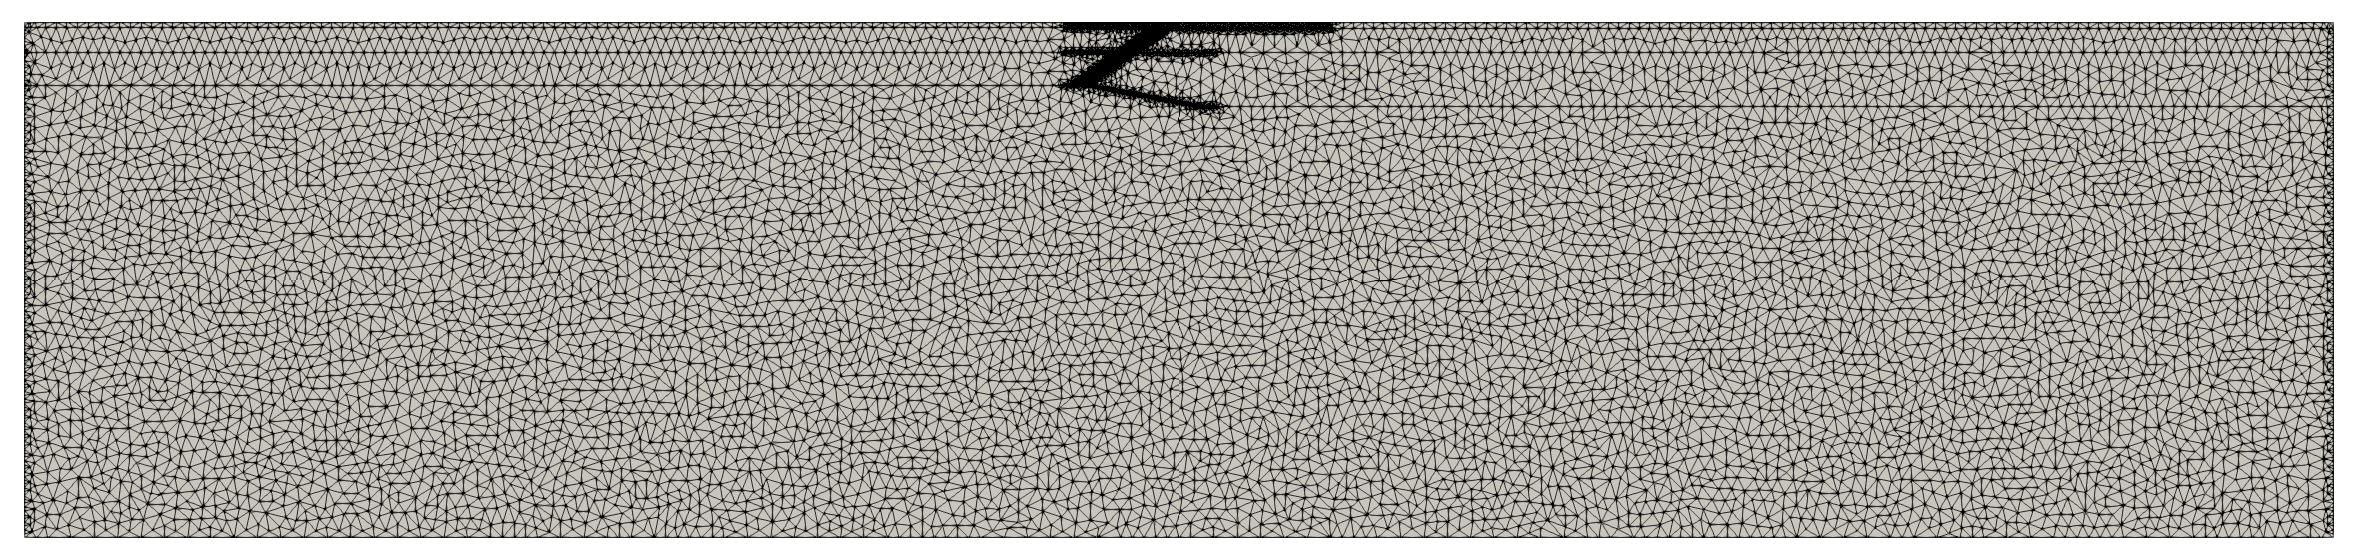
\includegraphics[width=12cm]{python_codes/fieldstone_127/results/mesh1}
%\end{center}

The rheology of the matrix can take several forms:
\begin{itemize}

%-------------------------
\item {\python rheology=0}: Constant viscosity $\eta=\SI{1e22}{\pascal\second}$. This renders
the physics linear (and independent of temperature). Changing the velocity boundary conditions
only changes the magnitude of the computed fields.

%-------------------------
\item {\python rheology=1}: Diffusion creep only, with $Q_{\rm df}=\SI{410e3}{\joule\per\mole}$, 
$A_{\rm df}=1e-7$, no activation volume.
\[
\eta_{\rm df}=A_{\rm df}^{-1}\exp \frac{Q_{\rm df}}{RT}
\]

%-------------------------
\item {\python rheology=2}: Diffusion creep of rheology 1 + $\tanh$ formulation from \textcite{gatt20} 

\begin{eqnarray}
\sigma &=& (a_0+b_0T) \left( 1+ \tanh( (a_1+b_1T)(\log_{10}(\dot\varepsilon_e)-(a_2+b_2T+c_2T^2)) )\right)\nn\\
\eta_{\rm tanh}&=&\frac{\sigma}{2 \dot{\varepsilon}_e} \nn
\end{eqnarray}

%-------------------------
\item {\python rheology=3}: Diffusion creep of rheology 1 + erf formulation from \textcite{gatt20} 


\begin{eqnarray}
\sigma &=&(a_0+b_0T) \left( 1+ {\rm erf}( (a_1+b_1T)(\log_{10}(\dot\varepsilon_e)- (a_2+b_2T+c_2T^2)) )  
\right) \nn\\
\eta_{\rm erf}&=&\frac{\sigma}{2 \dot{\varepsilon}_e} \nn
\end{eqnarray}


%-------------------------
\item {\python rheology=4}: Diffusion creep of rheology 1 + Dislocation creep from \textcite{gocg19} (2019):
\[
\eta_{\rm ds} = A_{\rm ds}^{-1/n} \dot\varepsilon_e^{-1+1/n_{\rm ds}}
\exp\left( \frac{Q_{\rm df}}{n_{\rm ds}RT} \right)
\]
with $A_{\rm ds}=5.27e-29$, $n_{\rm ds}=4.5$, $Q_{\rm ds}=443e3$.

%-------------------------
\item {\python rheology=5}: Diffusion creep of rheology 1 + Dislocation creep from \textcite{gatt20} (2020):
\[
\eta_{\rm ds} = A_{\rm ds}^{-1/n} \dot\varepsilon_e^{-1+1/n_{\rm ds}}
\exp\left( \frac{Q_{\rm df}}{n_{\rm ds}RT}\right)
\]
with $A_{\rm ds}=5e-16$, $n_{\rm ds}=3.5$, $Q_{\rm ds}=540e3$.


\end{itemize}


WRITE about multivalued fields on nodes.

%\newpage
%------------------------------------------------------------------------------
%\subsection*{Results - rheology=0}

%\begin{center}
%\includegraphics[width=8cm]{python_codes/fieldstone_127/results/rheo0/u}
%\includegraphics[width=8cm]{python_codes/fieldstone_127/results/rheo0/v}\\
%\includegraphics[width=8cm]{python_codes/fieldstone_127/results/rheo0/press}
%\includegraphics[width=8cm]{python_codes/fieldstone_127/results/rheo0/eta}\\
%\includegraphics[width=8cm]{python_codes/fieldstone_127/results/rheo0/sr}
%\end{center}

%\newpage
%------------------------------------------------------------------------------
%\subsection*{Results - rheology=1}

%\begin{center}
%\includegraphics[width=8cm]{python_codes/fieldstone_127/results/rheo1/u}
%\includegraphics[width=8cm]{python_codes/fieldstone_127/results/rheo1/v}\\
%\includegraphics[width=8cm]{python_codes/fieldstone_127/results/rheo1/press}
%\includegraphics[width=8cm]{python_codes/fieldstone_127/results/rheo1/eta}\\
%\includegraphics[width=8cm]{python_codes/fieldstone_127/results/rheo1/sr}
%{\captionfont sr -14, T=1400}
%\end{center}

%\newpage
%------------------------------------------------------------------------------
%\subsection*{Results - rheology=2}

%\newpage
%------------------------------------------------------------------------------
%\subsection*{Results - rheology=3}


